\chapter{Design} \label{chapter:design}
This chapter of the report has the purpose of presenting the architecture of the DC-Net simulator from different perspectives through the utilization of UML diagram notations.

Firstly, I explain the reasons behind the design choices taken. Secondly, the architecture of the simulator is presented, also showing an example of how the event-based communication happens. Lastly, there is a series of sequence diagrams that exemplifies the data flow between clients and server both for the basic implementation of the protocol and the advanced one. \newline

Throughout the chapter some of the technologies are named, which will be presented in the implementation section (chapter \ref{chapter:implementation}).


\section{Design Choices}
Throughout the project, a number of decisions about the design of the simulator architecture were taken. This sections gi

The simulation will be a real-time web-based application that resembles the dynamics of the Dining Cryptographers. The simulation also attempts to be as faithful as possible to the original protocol to preserve untraceability.


I deem choice of a web application appropriate for three reasons:
\begin{enumerate}
    \item From a user perspective, downloading and installing the application and its third-party required components (dependencies) is likely to end up in technical issues. By using a website, the user can focus on learning the protocol rather than having to overcome possible set-up barriers of a native application;
    \item Building a website entails creating a Graphical User Interface (GUI). This results in a more user-friendly experience in respect to a command line application, often the interface of choice for most of the DC-Net simulations available.
    \item A live web application allows clients to connect to the DC-Net server over the internet. Such distributed architecture is a realistic implementation of the protocol. This represents an important step forward in comparison to the of the other simulations I found. In fact, as observed in section \ref{sec:similarWorks}, current simulations often employ scripts to emulate all the nodes on the same machine.
\end{enumerate}

The website will employ a client-server architecture. This design is considered appropriate for the simulation since it offers a farther reach to build complex mechanisms for handling the advanced requirements.

\textbf{It is important to highlight that the software implemented is going to be a \emph{simulation}. The role of the server in the application is seen as a facilitator to exchange messages between clients. Therefore, addressing the trust issue mentioned in section \ref{sec:clientserver} is beyond the scope of this project.}

A ring topology is the key exchange graph employed.


To ensure the secure exchange of keys, 




\subsection{Collision warning necessity}
Moreover, I set up a collision detection warning, which is a notification sent by the server only to the participants who attempted but failed to win a voting round. 

This mechanism has been implemented to avoid the necessity to send a unicast 'success' notification to the winning participant of the voting round, which would obviously uncover who the message sender is to a potential eavesdropper.


self-declared status. 
A participant trying to win the voting round automatically declares himself the message sender on his browser, as if he were successful in the round. 


In fact, if all participants tried to win the voting round the communication is aborted.


\section{System Architecture}
The architecture of the simulator is simple. Only server and client are present in the picture and there is no persistent data to be stored in a database. The communication between back-end and front-end happens through socket.io events.

\begin{figure}[H]
    \centering
    \fbox{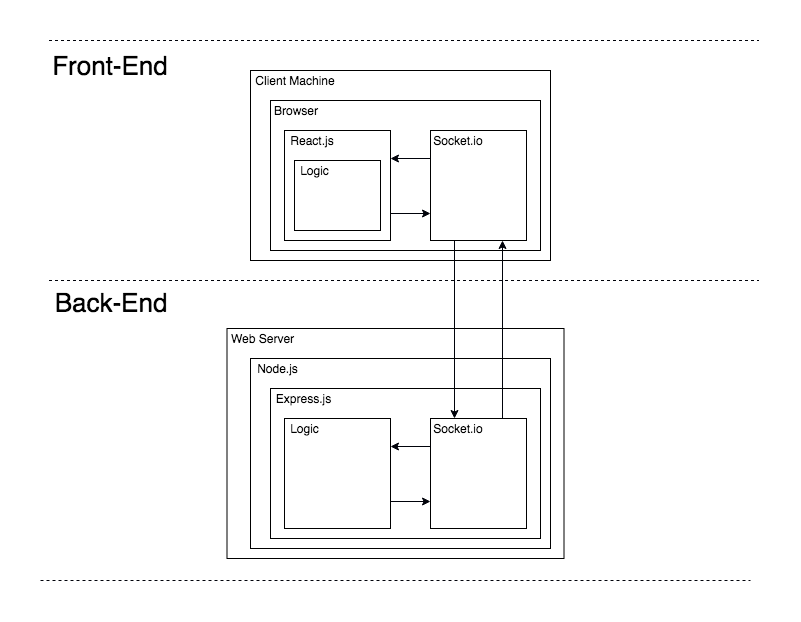
\includegraphics[width=0.9\textwidth]{Images/Design/architecture.png}}
    \caption{System Architecture}
    \label{fig:systemArchitecture}
\end{figure}



\section{Minimal Distributed Architecture}

\begin{figure}[H]
    \centering
    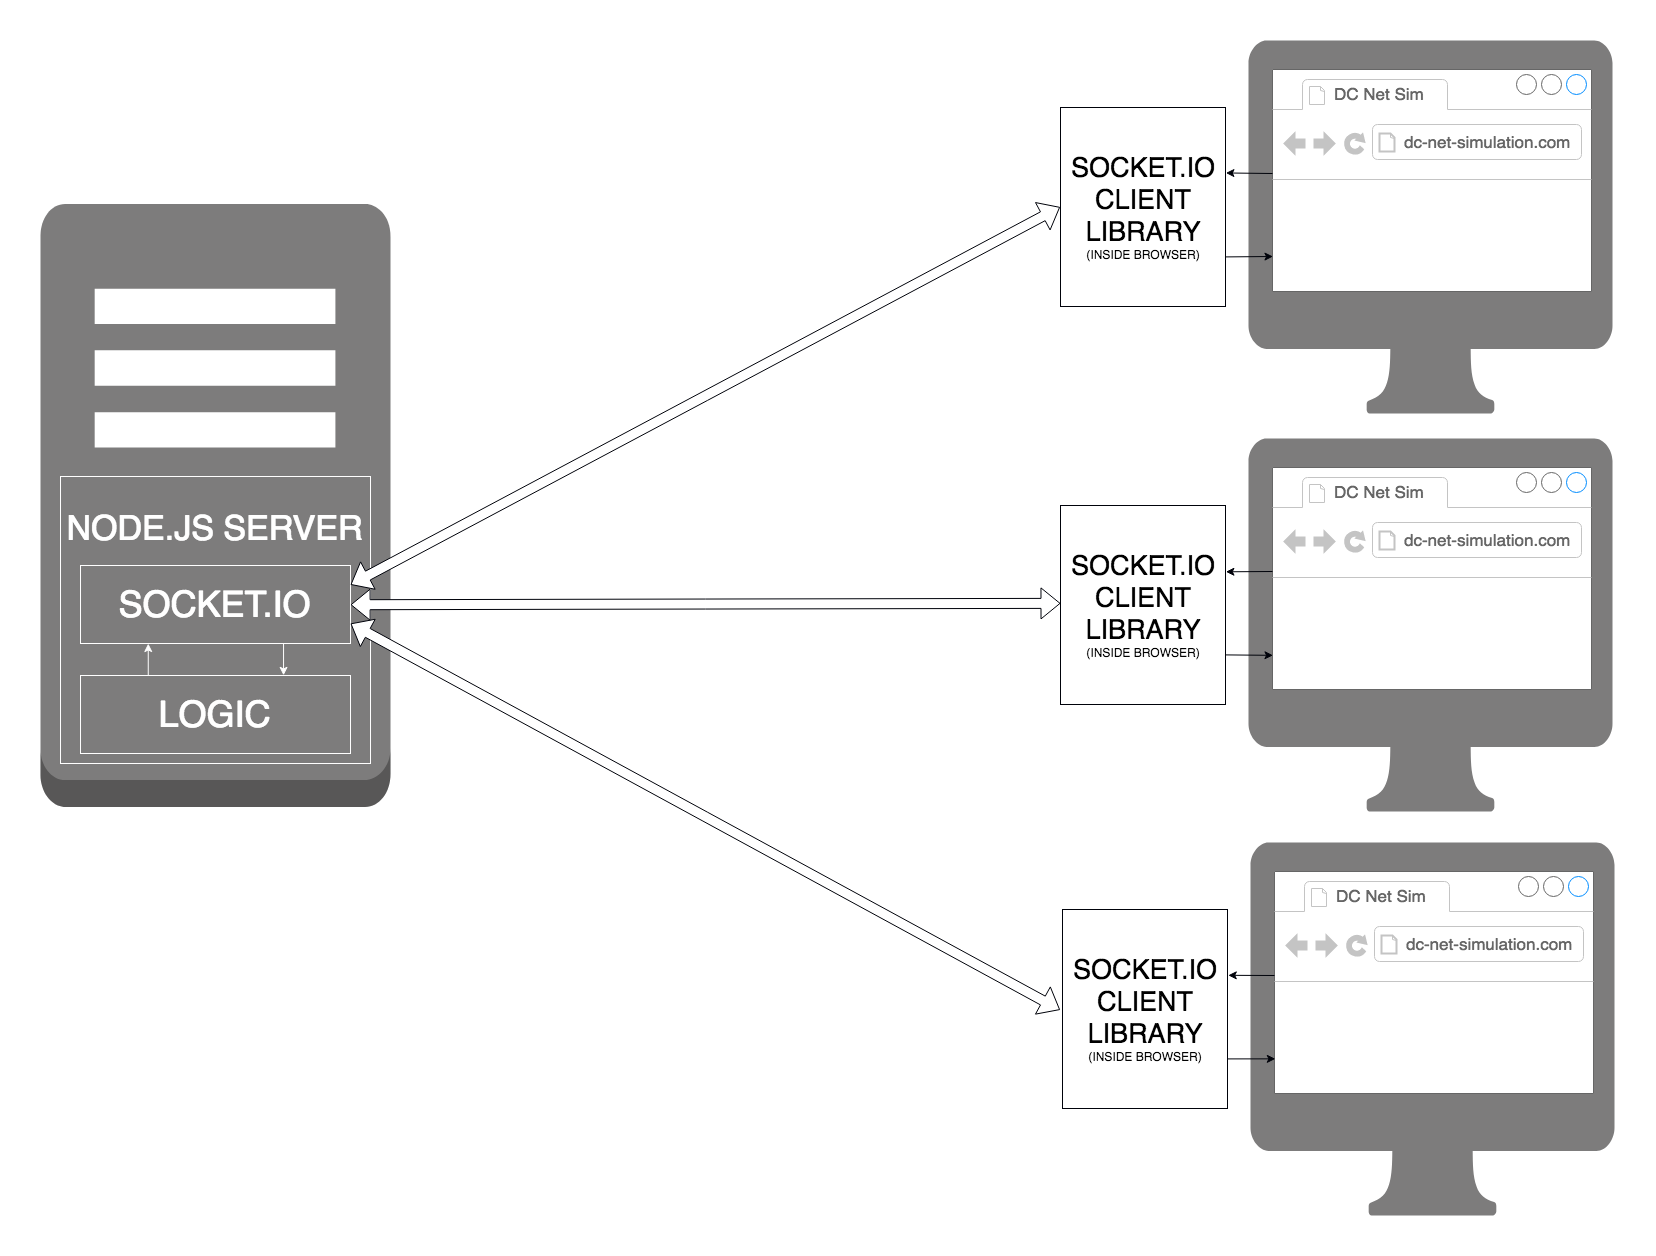
\includegraphics[width=0.8\textwidth]{Images/Design/distributedArchitecture.png}
    \caption{Server with three clients connected}
    \label{fig:distrubtedArchitecture}
\end{figure}


\section{Event-Based Communication Example}
View from single client point of view.

\begin{figure}[H]
    \centering
    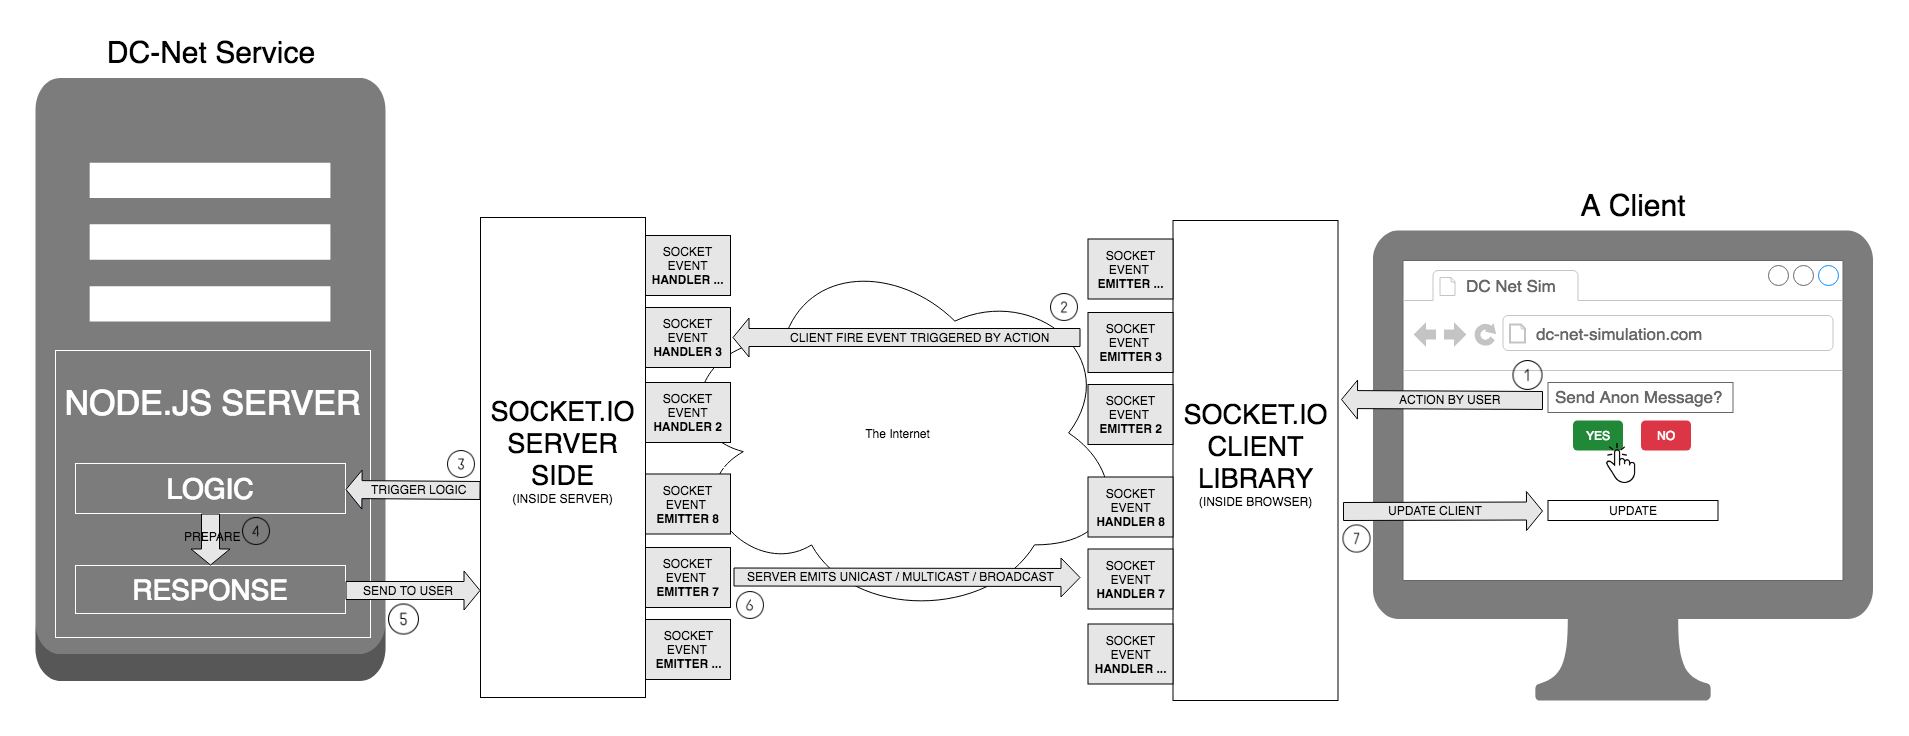
\includegraphics[width=1\textwidth]{Images/Design/singleClientSocketEvent.png}
    \caption{Socket event emission from client example}
    \label{fig:socketEventEmission}
\end{figure}



\section{Data flow depiction through sequence diagrams}


\begin{figure}[H]
    \centering
    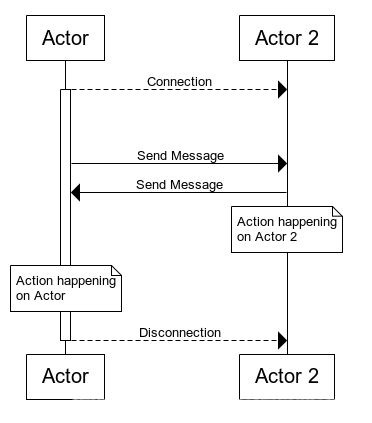
\includegraphics[width=0.5\textwidth]{Images/Design/seqDiagramLegend.png}
    \caption{Sequence Diagram Legend}
    \label{fig:sequenceDiagramLegend}
\end{figure}


\subsection{Basic Data Flow Design}

\begin{figure}[H]
    \centering
    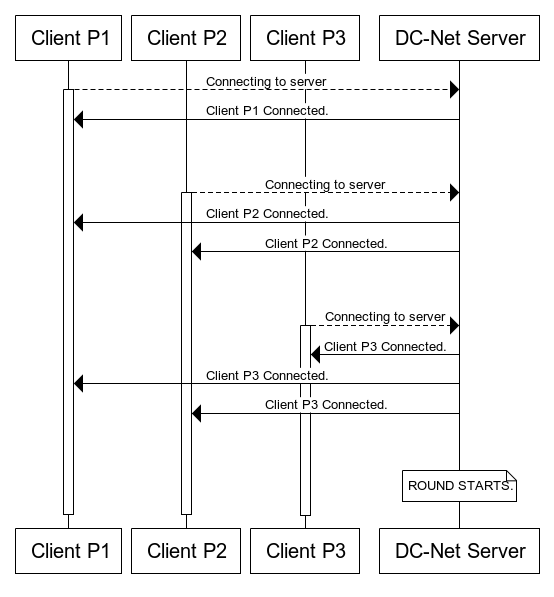
\includegraphics[width=0.7\textwidth]{Images/Design/clientsConnection.png}
    \caption{Connection of three clients needed to start protocol}
    \label{fig:clientsConnection}
\end{figure}

\begin{figure}[H]
    \centering
    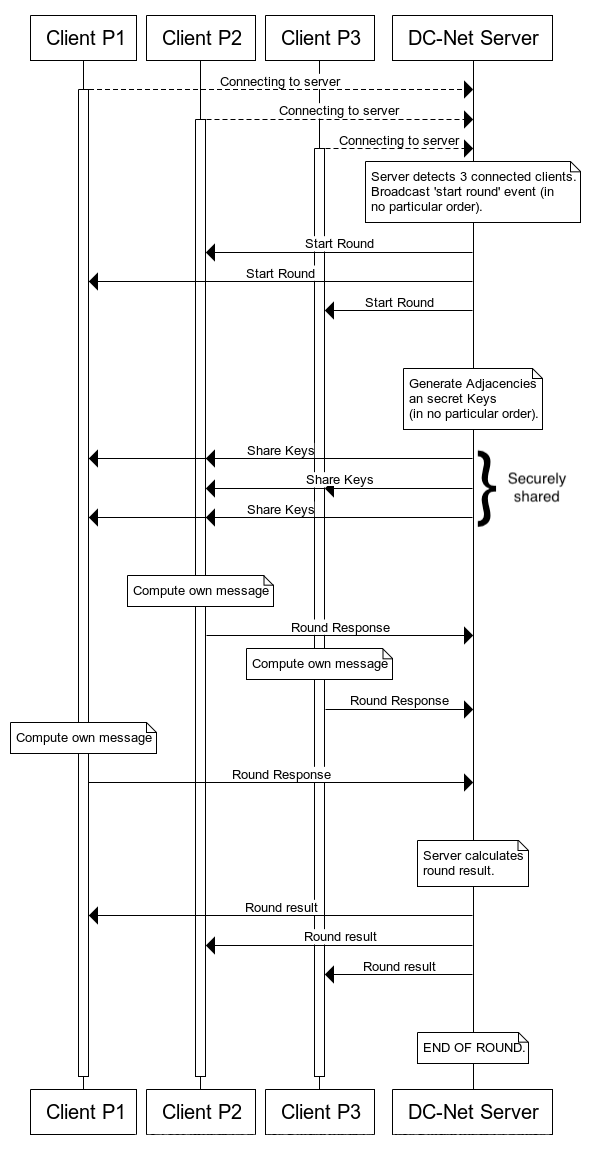
\includegraphics[width=0.8\textwidth]{Images/Design/successfulRound.png}
    \caption{Detailed example of a successful round}
    \label{fig:successfulRound}
\end{figure}

\begin{figure}[H]
    \centering
    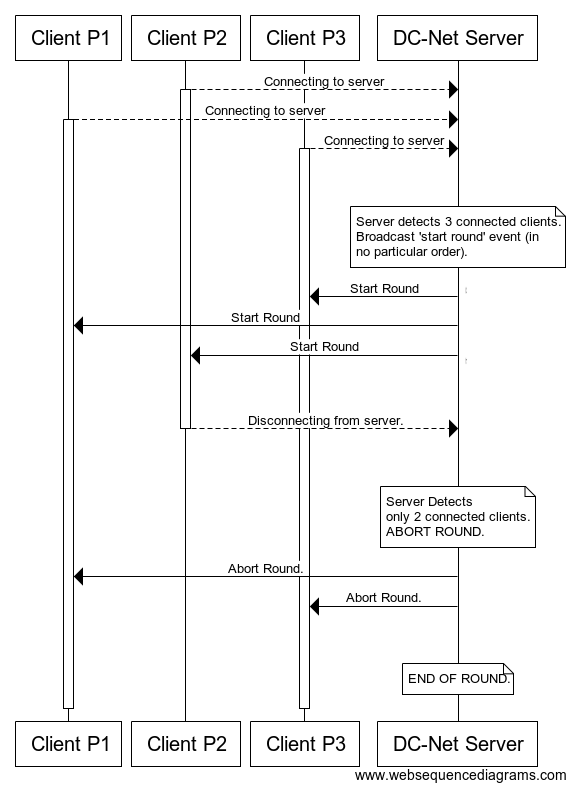
\includegraphics[width=0.7\textwidth]{Images/Design/abortedRound.png}
    \caption{Detailed example of aborted round}
    \label{fig:abortedRound}
\end{figure}

\begin{figure}[H]
    \centering
    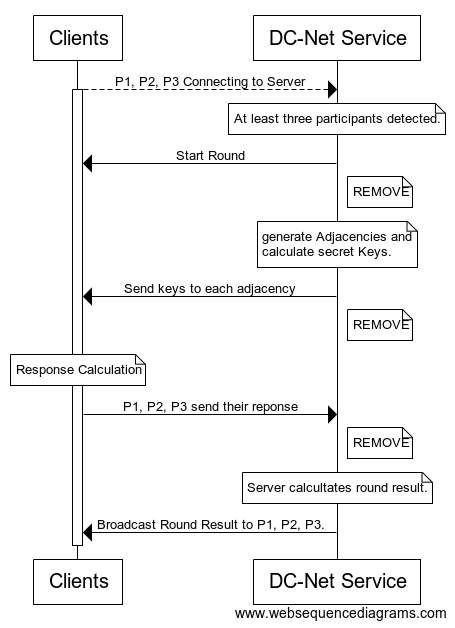
\includegraphics[width=0.7\textwidth]{Images/Design/singleRoundCondensed.png}
    \caption{Concise representation of a single round }
    \label{fig:singleRoundCondensed}
\end{figure}


\subsection{Advanced Data Flow Design}


\begin{figure}[H]
    \centering
    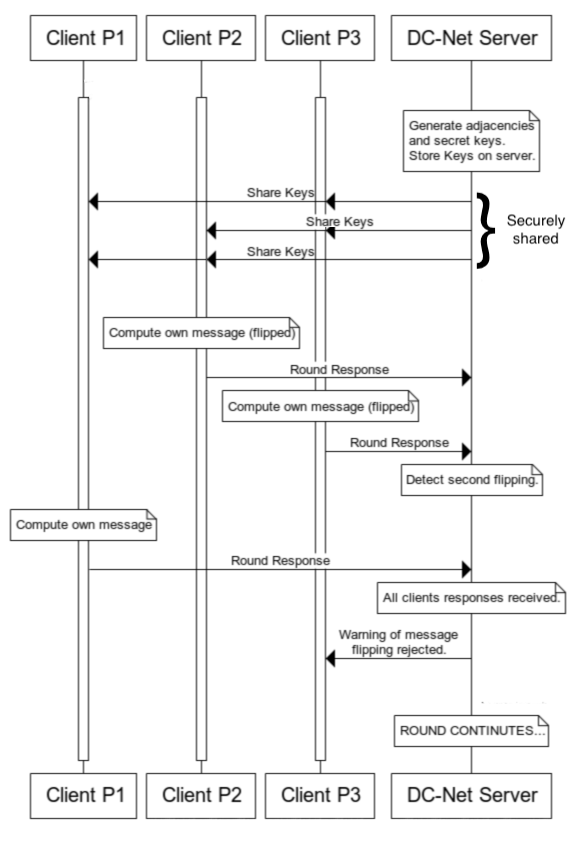
\includegraphics[width=0.6\textwidth]{Images/Design/collisionDetection.png}
    \caption{Detecting message collision}
    \label{fig:collisionDetection}
\end{figure}

\begin{figure}[H]
    \centering
    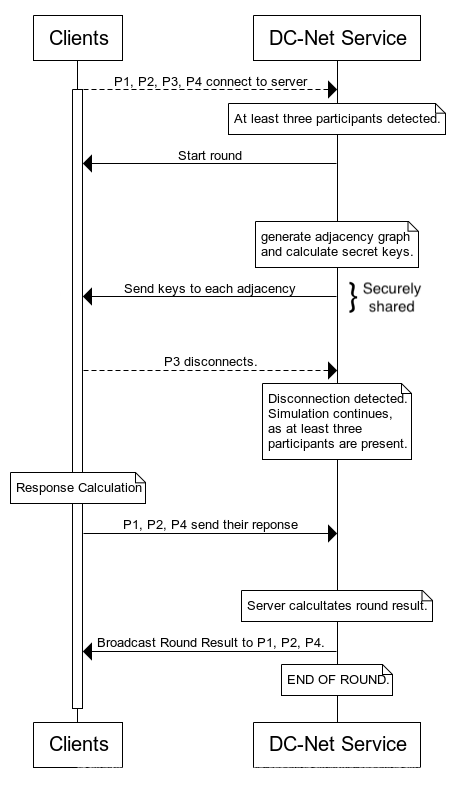
\includegraphics[width=0.5\textwidth]{Images/Design/roundWithDisconnections.png}
    \caption{Round performed with disconnecting client}
    \label{fig:roundWithDisconnections}
\end{figure}

\begin{figure}[H]
    \centering
    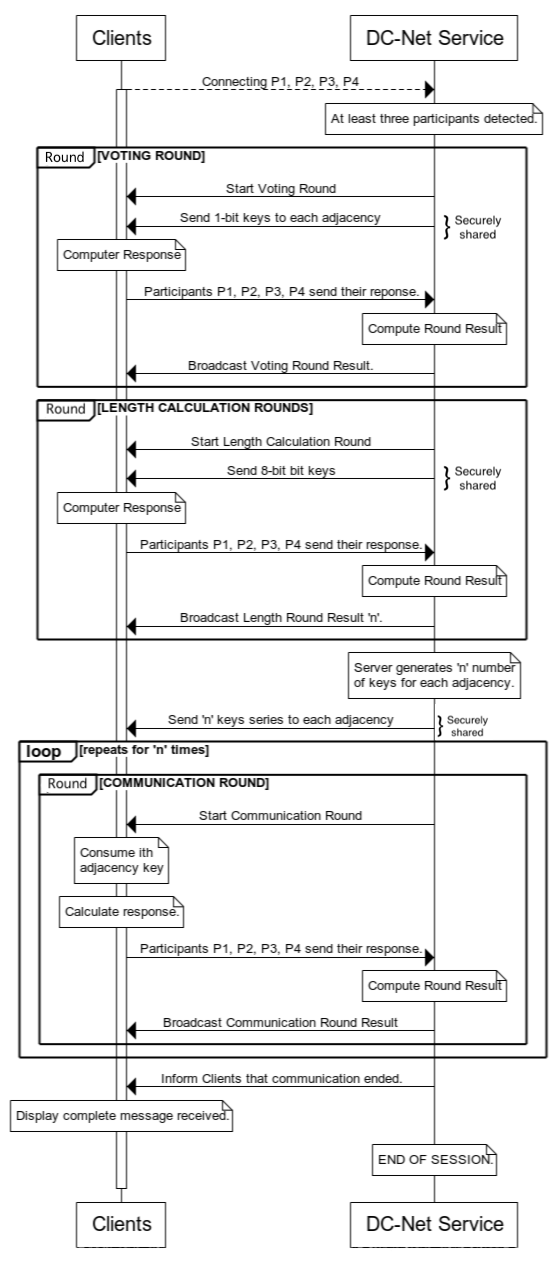
\includegraphics[width=0.6\textwidth]{Images/Design/longRound.png}
    \caption{Representation of complex round of communication}
    \label{fig:longRound}
\end{figure}